\documentclass[8pt]{extarticle}
% Font
\usepackage[default]{opensans}
\linespread{1.25}
% Margins
\usepackage[top=30mm,bottom=18mm,left=18mm,right=18mm]{geometry}
% Graphics and images
\usepackage{graphicx}
% Encodings (to render letters with diacritics and special characters)
\usepackage[utf8]{inputenc}
\usepackage[T1]{fontenc}
% Language
\usepackage[portuguese]{babel}
% Hyperreferences
\usepackage{hyperref}
\hypersetup{
    colorlinks=true,
    linkcolor=blue,
    filecolor=magenta,      
    urlcolor=blue,
}
\urlstyle{same}
% Headers and footers
\usepackage{fancyhdr}
\pagestyle{fancyplain}
\fancyhf{}
\lhead{Diogo Miguel Ferreira Rodrigues}
\rhead{\thepage}
% Subsections
\usepackage{titlesec}
\titleformat{\subsection}{\large}{\thesubsection}{}{\scshape}
\titlespacing*{\subsection}{0pt}{0pt}{0.6\baselineskip}
% Commands
%\usepackage{showframe}
%% Parag
\newcommand{\parag}[1]{
\begin{minipage}{\textwidth} \hfill
\begin{minipage}{\dimexpr\textwidth-0.6cm}
	#1
\end{minipage}
\end{minipage}
}
%% Itemtime
\newcommand{\itemtime}[2]{
#1 \hfill \begin{minipage}[t]{0.185\textwidth}         #2  \end{minipage}
}
%% Job
\newcommand{\job}[3]{\parag{
\itemtime{\textbf{#1}}{\textbf{#2}}\\
#3 \vspace*{9px}}}
%% Pub
\newcommand{\pub}[3]{\parag{
\itemtime{\textit{#1}}{#2}\\
#3 \vspace*{9px}}}
%% Idiom
\newcommand{\idiom}[2]{\textbf{#1} – #2\vspace*{6px}\\}
% Document
\begin{document}
\thispagestyle{empty}
\noindent
\begin{minipage}[l]{0.75\textwidth}
	\section*{Diogo Miguel Ferreira Rodrigues}
	Rua de Avioso, 553 | Castêlo da Maia (4475-617 MAIA)\\
    \begin{tabular}{@{}c @{\hskip 0.5em} l @{\hskip 5em} c @{\hskip 0.5em} l @{}}
        
\includegraphics[height=7px]{email.png}    & \href{mailto:diogo.rodrigues@fe.up.pt}{diogo.rodrigues@fe.up.pt}     & 
\includegraphics[height=7px]{linkedin.png} & \href{https://www.linkedin.com/in/dmfrodrigues/}{dmfrodrigues} \\
                                                   & \href{mailto:dmfrodrigues2000@gmail.com}{dmfrodrigues2000@gmail.com} & 
\includegraphics[height=7px]{github.png}   & \href{https://github.com/dmfrodrigues}{dmfrodrigues}\\
        
\includegraphics[height=7px]{phone.png}    & +351 915507239 \\
    \end{tabular}
\end{minipage}%
\write18{ curl -L https://i.imgur.com/EdhdoGQ.jpg --output cv_photo.jpg ; }
\begin{minipage}[l]{0.24\textwidth}
	\begin{center} 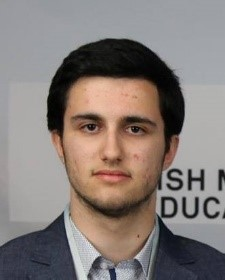
\includegraphics[height=30mm]{cv_photo.jpg} \end{center}
\end{minipage}
\subsection*{Educação}
\job{Mestrado Integrado em Engenharia Informática e Computação}{2018 – 2023}{
Faculdade de Engenharia da Universidade do Porto\\
Conclusão do 2º ano com classificação global do curso 19.05/20.00
}
\job{Ensino Secundário – Curso Científico-Humanístico de Ciências e Tecnologias (10º-12º anos)}{2015 – 2018}{
Escola Secundária do Castêlo da Maia\\
Conclusão com média 19.6/20.0\\
Prémio de Mérito do Ministério da Educação, por melhor classificação do estabelecimento escolar
}
\subsection*{Cargos \& experiência}
\job{Assistente de Investigação}{2019 – 2020}{
INESC-TEC – Laboratório de Inteligência Artificial e Apoio à Decisão (LIAAD)\\
\textit{Research on European Children and Adults Born Preterm} (RECAP)
}
\job{Membro do Comité Científico das \textit{Olimpíadas Nacionais de Informática – ONI}}{2018 – }{
Convidado na condição de ex-participante nas \textit{Olimpíadas Nacionais de Informática} e nas \\
\mbox{\textit{Olimpíadas Internacionais de Informática}}
}
\subsection*{Competências}
\parag{
\textbf{Linguagens de programação:}\\
Nível avançado: C/C++, Python, Javascript, MATLAB, makefile\\
Nível intermédio: PHP, R, GNU Bash, SQL (SQLite)\\
Nível fundamental: Assembly (ARMv7, ARMv8), Visual Basic\\ 
\textbf{Tecnologias:}\\
Git: controlo de versões, branching, submódulos\\
Github: issues, projects, actions/workflows\\
Tecnologias web: NodeJS, cURL, pedidos HTTP por Ajax e XHR\\
\textbf{Outras competências:}\\
Elaboração de documentos em LaTeX e Markdown\\
Terminais Unix, GNU Bash shell\\
Sistemas operativos Linux (Ubuntu)
}
\subsection*{Publicações \& artigos}
\pub{AI Approach to Population Demographics using Satellite Imagery}{2019}{
\textit{London International Youth Science Forum 2019}\\
Apresentação financiada pela Fundação Calouste Gulbenkian
}
\subsection*{Bolsas}
\job{Bolseiro Gulbenkian}{24-07-2019 – 07-08-2019}{
Participação no \textit{London International Youth Science Forum 2019}\\
Imperial College London \& Royal Geographical Society, Londres\\
Apresentação de trabalho em formato poster\\
Participação financiada pela Fundação Calouste Gulbenkian
}
\subsection*{Voluntariado}
\job{\textit{European Union Science Olympiad 2019 – Almada}}{04-05-2019 – 11-05-2019}{
Guia das equipas \textit{Italy A} e \textit{Italy B} na \textit{European Union Science Olympiad 2019}, em Almada e Lisboa\\
Organização da EUSO e acompanhamento dos alunos participantes na competição durante a semana, garantindo o seu bem-estar e providenciar o apoio necessário aos alunos estrangeiros, nomeadamente na facilitação da sua estadia em Portugal com traduções para inglês e contextualização sociocultural durante os eventos.
}
\subsection*{Competições \& medalhas}
\job{\textit{Prémio Incentivo a estudantes distintos} da Universidade do Porto}{2018/19}{
Atribuído pela Universidade do Porto a estudantes distintos em primeiro ano de matrícula.\\
Pela obtenção da classificação média de 19.03/20.00 no final do 1º ano de curso\\
Melhor classificação da Faculdade de Engenharia da Universidade do Porto\\
2ª melhor classificação da Universidade do Porto
}
\job{Participação no \textit{SouthWestern Europe Regional Contest – SWERC2019-20}}{24-01-2020 – 27-01-2020}{
Institut Polytechnique de Paris, Paris, França\\
40º lugar na classificação geral
}
\job{1º lugar na \textit{Competição de Programação da Semana de Informática 2019}}{27-10-2019 – 30-10-2019}{
Faculdade de Engenharia da Universidade do Porto
}
\job{6º lugar na \textit{Maratona Inter-Universitária de Programação – MIUP2019}}{12-10-2019}{
Instituto Superior Técnico, Lisboa
}
\job{Participação no \textit{SouthWestern Europe Regional Contest – SWERC2018} (\textit{ICPC2018})}{01-12-2018 – 02-12-2018}{
Télécom ParisTech, Paris, França\\
33º lugar na classificação geral
}
\job{1º lugar na \textit{Competição de Programação da Semana de Informática 2018}}{29-10-2018 – 01-11-2018}{
Faculdade de Engenharia da Universidade do Porto
}
\job{Medalha de Bronze na \textit{Maratona Inter-Universitária de Programação – MIUP2018}}{13-10-2018}{
Departamento de Informática da Universidade da Beira Interior, Covilhã\\
4º lugar na classificação geral
}
\job{Participação na \textit{30th International Olympiad in Informatics – IOI2018}}{01-09-2018 – 08-09-2018}{
Tsukuba, Ibaraki, Japão
}
\job{Menção Honrosa na \textit{49th International Physics Olympiad – IPhO2018}}{21-07-2018 – 29-07-2018}{
Lisboa, Portugal\\
2º lugar de entre os alunos portugueses, 226º na classificação global
}
\job{7º lugar nacional na Final Nacional das \textit{Olimpíadas Nacionais de Informática – ONI2018}}{07-05-2018}{
Departamento de Ciência de Computadores – Faculdade de Ciências da Universidade do Porto\\
Convidado para participar no estágio de preparação para a \textit{International Olympiad in Informatics 2018}
}
\job{Medalha de Prata na \textit{European Union Science Olympiad 2017 – Copenhagen}}{07-05-2017 – 14-05-2017}{
6º lugar na classificação global – Medalha de Prata\\
Provas realizadas na \textit{University of Copenhagen} e na \textit{Technical University of Denmark}
}
\job{Medalha de Ouro nas \textit{Olimpíadas Nacionais de Física 2015}}{05-06-2015 – 06-06-2015}{
Museu da Eletricidade (atualmente MAAT – Museu de Arte, Arquitetura e Tecnologia), Lisboa\\
Categoria A (até 9º ano)\\
Convite para participar na seleção para a \textit{European Union Science Olympiad 2017 – Copenhagen}
}
\job{Medalha de Bronze na Final Nacional das \textit{XXXIII Olimpíadas Portuguesas de Matemática}}{19-03-2015 – 22-03-2015}{
Escola Secundária Dr. Augusto César da Silva Ferreira, Rio Maior\\
Categoria A (8º/9º anos)\\
Convidado para participar no Projeto Delfos
}
\subsection*{Fóruns, palestras, conferências \& congressos}
\job{\textit{London International Youth Science Forum 2019}}{24-07-2019 – 07-08-2019}{
Imperial College London \& Royal Geographical Society, Londres\\
Apresentação de trabalho em formato poster\\
Participação financiada pela Fundação Calouste Gulbenkian
}
\subsection*{Idiomas}
\parag{
\idiom{Português}{idioma nativo}
\idiom{Inglês}{falante fluente (C1), proficiente na leitura (C1) e escrita (C1) sobre assuntos complexos}
\idiom{Espanhol}{intermédio na fala (B2), leitura (B2) e escrita (B1)}
\idiom{Francês}{falante elementar (A2), intermédio na leitura (B2) e escrita (B1)}
}
\subsection*{Associações \& projetos}
\job{\textit{Research on European Children and Adults Born Preterm} (RECAP)}{Set/2018 – Mar/2019}{
O objetivo do projeto RECAP Preterm é melhorar a saúde, o desenvolvimento e a qualidade de vida de crianças e adultos nascidos prematuros na União Europeia, através do desenvolvimento da \textit{RECAP Preterm Cohort Platform}, uma base de dados sustentável, geograficamente diversa e multidisciplinar de \textit{cohorts} nacionais e Europeus de bebés muito prematuros ou com peso à nascença muito baixo, constituídos ao longo de 30 anos e desenhados de forma a otimizar a utilização de dados populacionais para investigação e inovação nas áreas da saúde, social e de educação.
}
\job{Comunidade FEUP-SWERC}{2018 – }{
Comunidade colaborativa de alunos e professores da Faculdade de Engenharia da Universidade do Porto, com o objetivo de disseminar o gosto pela programação competitiva na comunidade FEUP, dinamizar competições de programação e selecionar/preparar os alunos da Faculdade para representação em competições de programação nacionais, europeias e internacionais.
}
\end{document}
